
\chapter{Background}
\textit{This chapter serves two main purposes. Firstly, it evaluates the available literature surrounding the effectiveness of techniques for modelling, control and state estimation in unmanned aerial vehicles and related platforms. Secondly, it introduces the key mathematical, physical and technical concepts necessary for the discussion in the following chapters.}

\section{Modelling Multi-Rotor Vehicles}
\subsection{Modelling Approaches}
In order to control a system, it is first necessary to have an understanding of the dynamics of the system. There are multiple methods used for developing mathematical models in order to describe the dynamics of multi-rotor vehicles. The Newtonian approach uses forces and torques in order to describe the system, whereas the Lagrangian approach utilises energies \cite{Raine2017}.\\

 Further, attitude of the vehicle can be described by using either Euler angles or quaternions. Euler angles express attitude with three angles, each representing the rotation in 3D space around each axis. Alternatively, quaternion algebra is used to represent attitude with four scalar variables representing a point on the unit sphere \cite{Voight2021}. Euler representation is more intuitive, however quaternion representation has the advantage of avoiding a problem known as gimbal lock which arises when two of the Euler rotation axes align, resulting in a loss of a degree of freedom.\\

Newton-Euler formalism combines Newtonian mechanics and Euler angle representation in order to describe the rotational and translational dynamics of rigid bodies. This approach is commonly used to develop a mathematical model for multi-rotor vehicles. The main advantage of this method is that it is simple to understand. Alternatively, using Euler-Lagrange formalism results in a more compact derivation \cite{Zhang2014}. \\

Multiple studies demonstrate the effectiveness of multi-rotor models developed using Newton-Euler formalism \cite{Bouabdallah2006}, \cite{Baranek2012}. Therefore, this thesis will utilise this method. Due to the uncomplicated nature of this formulation, identifying issues in the model and debugging simulations will, in general, be easier as compared to similar models formed using quaternion algebra or Lagrangian techniques.



\subsection{Newton-Euler Equations}
The Basic Kinematic Equation (BKE) is used in Newton-Euler dynamics to describe the relative motion of two reference frames \cite{Ardema2006}. The BKE is given in Equation \ref{eqn:BKE1}:
\begin{equation}\label{eqn:BKE1} 
\frac{d\textbf{Q}_{a}}{dt}=\frac{d\textbf{Q}_{b}}{dt}+\mathbf{\omega}_{b} \times \textbf{Q}_{b}
\end{equation}
where $\textbf{Q}_{a}$ and $\textbf{Q}_{b}$ represent a three-dimensional quantity (e.g position, velocity) with respect to reference frames \{A\} and \{B\} respectively, and $\mathbf\omega_{b}$ represents the angular velocity of \{B\} with respect to \{A\}. Now, consider reference frame \{B\} to be fixed at the centre of mass of some rigid body. By considering the mass of the body and taking \textbf{Q} as the translational velocity of the body (\textbf{v}), the BKE (Equation \ref{eqn:BKE1}) can be written in terms of forces to give the first of the Newton-Euler equations.

\begin{equation*}
\begin{split} 
\frac{d\textbf{v}_{a}}{dt}&=\frac{d\textbf{v}_{b}}{dt}+\omega_{b} \times \textbf{v}_{b}\\
m\dot{\textbf{v}}_{a}&=m(\dot{\textbf{v}}_{b}+\omega_{b} \times \textbf{v}_{b})\\
\textbf{F}_{a}&=m(\dot{\textbf{v}}_{b}+\omega_{b}\times\textbf{v}_{b})
\end{split}
\end{equation*}

The moments of forces (torques) about the centre of mass may be considered in a similar way in order to produce the second of the Newton-Euler equations \cite{Ardema2006}:
\begin{equation*}
\textbf{M}_{b}=\textbf{I}_{b}\dot{\omega}_{b}+\omega_{b}\times\textbf{I}_{b}\omega_{b}
\end{equation*}
where $\textbf{M}_{b}$ represents the three-dimensional moment about \{B\}, and $\textbf{I}_{b}$ is a 3$\times$3 matrix representing the moment of inertia about the centre of mass.

\subsection{Reference Frames and Coordinate Systems}\label{section:RefFrames}
Establishing a model of an aerial vehicle requires an understanding of coordinate systems or reference frames and how they relate to given quantities (displacement, velocity, acceleration, etc). There are two main types of reference frames: inertial frames and non-inertial reference frames. An inertial reference frame is one which is not accelerating and within which Newton's laws are valid \cite{Nebylov2016}. On the other hand, a non-inertial reference frame is one which is experiencing acceleration.

There are many different reference frames which may be used to describe aircraft motion. For example, an Earth-fixed local frame is a reference frame with its origin fixed at an arbitrary point on the Earth. For the purposes of modelling an aerial vehicle, an Earth-fixed local frame can be considered as an inertial frame although it is experiencing acceleration due to the Earth's rotation. However, a reference frame which is fixed on the aircraft body is non-inertial as it experiences non-negligible acceleration due to the vehicle's movement. Rotation matrices enable the conversion of quantities between reference frames.

The most commonly used reference frame for Earth-based navigation identifies a position on the Earth in terms of latitudes and longitudes. In particular, GPS data is generally presented in this frame. Converting these global positions to displacements within a local reference frame can be done in a number of ways. The haversine formula is one such method, which considers two sets of coordinates and computes the displacement between them. The haversine formula arises from spherical trigonometry to compute the great-circle distance between two points on a sphere \cite{Smart1977}. The bearing ($\beta$) and distance (d) are given as:

\begin{equation}\label{eqn:haversine}
\begin{split}
d&=2R sin^{-1} \left( \sqrt{sin^{2}\left( \frac{\Delta\chi}{2} \right) +cos(\chi_{1})cos(\chi_{2})sin^{2} \left( \frac{\Delta\lambda}{2}  \right) }\right)\\
\beta&=atan2\left[ sin(\Delta\lambda)cos(\chi_{2}) , cos(\chi_{1})sin(\chi_{2}) - sin(\chi_{1}) cos(\chi_2) cos(\Delta\lambda)\right]
\end{split}
\end{equation}

where R is the Earth's radius, $\lambda_{1}$, $\chi_{1}$ represent the initial latitude and longitude coordinates respectively and $\lambda_{2}$, $\chi_{2}$ represent the final coordinates. $\Delta\lambda$ is equivalent to $(\lambda_{2}-\lambda_{1})$ and $\Delta\chi$ is equivalent to $(\chi_{2}-\chi_{1})$. The function $atan2(b,a)$ finds the angle between the positive x axis and the point defined by (a,b).
It is worth noting that this formula considers the Earth as a perfect sphere, when in reality it is elliptical to some extent. However, over short distances the effect of the Earth's elliptical nature on the accuracy of the results is negligible.


\section{Control Techniques}
%Effectiveness of different control techniques in drones from previous studies...
There are many control techniques both linear and nonlinear which have been employed to stabilise UAVs and allow position tracking. Two of the most common techniques - one linear technique and one nonlinear technique - will be explored in detail in this section. These are PID control (linear) and backstepping control (nonlinear). There are many other techniques which show promise for UAV control including (but not limited to) model predictive control (MPC), sliding-mode control, feedback linearisation, geometric techniques and learning-based control \cite{Rubi2019}. However, these will not be discussed in detail here.  
\subsection{Proportional Integral Derivative (PID) Control}\label{section:PIDBackground}
A PID control law consists of three terms each associated with a gain:

\[u(t)=K_{p}e(t)+K_{I}\int_{0}^{t}e(t)\,dt+K_{D}\frac{de(t)}{dt}\]
Where e(t) represents the measured error between the desired setpoint and the measured value of the variable. 

\begin{figure}[htb]
	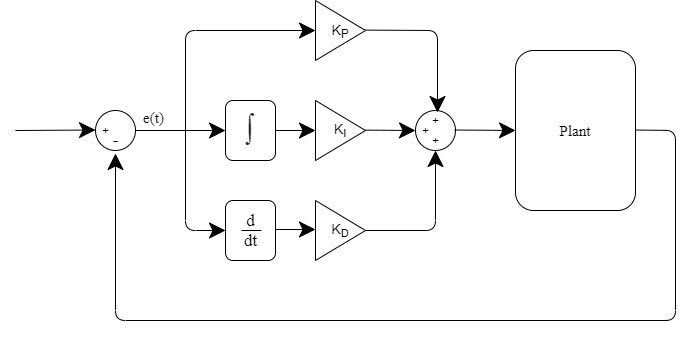
\includegraphics[width=\columnwidth]{PIDControl.png}%
	\caption{PID control block diagram.}%
	\label{fig:PIDControl}%
\end{figure}

PID control is comparatively simple compared to other techniques, but several studies suggest that it is generally effective for stabilising a UAV around a hovering setpoint, in the absence of large disturbances \cite{Bouabdallah2006}, \cite{Pounds2010}, \cite{Moussid2015}. \\

\subsection{Backstepping Control}\label{section:BacksteppingBackground}
The plant dynamics of a multi-rotor vehicle are inherently nonlinear, therefore nonlinear control techniques may be necessary to stabilise the vehicle. Backstepping control is a nonlinear recursive technique which is based upon Lyapunov stability. The mathematical background on the backstepping method in this section is largely based upon the work presented by Kokotovic \cite{1992a} and Krsti\'c et al. \cite{Krstic1995}.

\subsubsection{Lyapunov Stability}
Direct Lyapunov theorem, as stated in Appendix B of \cite{Isidori1995}, considers a time invariant system of the form:
\[\dot{x}=f(x)\]
with $x\in\mathbb{R}^{n}$, $f(x)$ is smooth and $f(0)=0$. If there exists a positive definite, proper and smooth function $V(x)$ which satisfies:
\[\frac{\partial V}{\partial x}f(x)<0\]
for all $x\neq0$, then the equilibrium of the system is globally asymptotically stable. This means that given any initial conditions, over time ($t\rightarrow\infty$) the system will approach its equilibrium point \cite{Chen1999}. 

Now, consider a time invariant nonlinear system with states $\mathbf{x}$ and inputs $\mathbf{u}$:
\begin{equation}\label{eqn:TISystem}
\mathbf{\dot{x}}=\mathbf{f}(\mathbf{x},\mathbf{u})
\end{equation}
with equilibrium at $\mathbf{x}=\mathbf{0}$. Following from Direct Lyapunov theorem, to stabilise such a system, a control law $\mathbf{u}=\mathbf{\alpha}(\mathbf{x})$ must be designed such that the equilibrium point of \eqref{eqn:TISystem} is globally asymptotically stable. To do this, a function $V(\mathbf{x})$ may be chosen as a candidate Lyapunov function. The control input, $\mathbf{\alpha}(\mathbf{x})$, must then be chosen such that $\dot{V}(\mathbf{x})=\frac{\partial V}{\partial \mathbf{x}}\mathbf{f}(\mathbf{x},\mathbf{\alpha}(\mathbf{x}))$ is negative definite for all $\mathbf{x}$. 

In order to apply this method to the tracking problem, the states of the system may be redefined as $\mathbf{z}=\mathbf{x}_{d}-\mathbf{x}$, where $\mathbf{x}_{d}$ represents the desired value of the states.

\subsubsection{Strict Feedback Form}
Backstepping control is best demonstrated on a system in strict feedback form \cite{1992a}. Consider the system:
\begin{equation*}
\begin{split}
\dot{x}_{1}&=f_{1}(x_{1},x_{2})\\
\dot{x}_{2}&=x_{3}+f_{2}(x_{1},x_{2})\\
\dot{x}_{3}&=u +f_{3}(x_{1},x_{2}, x_{3})
\end{split}
\end{equation*}

Now consider that $x_{2}$ can be used as a "virtual control" to stabilise $\dot{x}_{1}$, by choosing an appropriate Lyapunov function $V_{1}(x_{1})$. We will denote the virtual control (or desired value of the state) with a subscript 'd', e.g. $x_{2d}(x_{1})$ denotes the desired value of $x_{2}$. It is worth noting that although this is a function of $x_{1}$, it will henceforth be written as $x_{2d}$ for simplicity. Likewise for other virtual controls.  Now consider the error between the desired and actual values: $z_{2}=x_{2}-x_{2d}$. As we are considering the stabilisation problem, $x_{1d}=0$ and therefore $z_{1}=x_{1}$. To stabilise $z_{1}$, the virtual control $x_{2d}$ must be chosen such that the Lyapunov function $V_{1}(z_{1})$ has a negative time derivative.

Likewise, $x_{3}$ may be used to stabilise $z_{2}$ with a virtual control ($x_{3d}(z_{1},z_{2})$). A third error term is defined: $z_{3}=x_{3}-x_{3d}$. Also, a second Lyapunov function is defined: 
\begin{equation*}
V_{2}(z_{1},z_{2})=V_{1}(z_{1})+\frac{1}{2}z_{2}^{2}
\end{equation*}
The feedback law $x_{3d}$ is chosen such that the time derivative of this Lyapunov function is negative. 

The final iteration for this system is complete by choosing the actual control $u$ to stabilise $z_{3}$. Again, this is done in the same way by defining a third Lyapunov function:
\begin{equation*}
V_{3}(z_{1},z_{2},z_{3})=V_{2}(z_{1},z_{2})+\frac{1}{2}z_{3}^{2}
\end{equation*}
The control input $u$ is then chosen such that the time derivative is negative definite. This results in global asymptotic stability of the system at the equilibrium point. Thus, the entire system is stabilised by the single control input ($u$) by the recursive backstepping of virtual control inputs ($x_{2d}$, $x_{3d}$). This concept is able to be applied to control the position of multi-rotor aircraft, by using the Euler angle values as virtual controls.


\subsubsection{Implementation in UAV Control}

Numerous studies have investigated various implementations of backstepping control strategies both in simulation and on physical UAV platforms. This control method is flexible and variations on the control law will arise depending on the design decision to cancel or retain nonlinearities. Also, the specific UAV platform and the modelling method used to describe the system can result in differences between the derived control laws.

Backstepping control systems for multi-rotor UAVs are simulated with successful results in many studies. \cite{Mian2008} demonstrates stabilisation of the rotational subsystem of a quadrotor using a backstepping control law, with the translational subsystem controlled using PID. \cite{ArellanoMuro2013} demonstrates satisfactory simulation results for trajectory tracking of a quadrotor in the presence of external disturbances. \cite{Roza2012} presents similar results with a controller that allows a speed profile and yaw angle to be specified as a function of displacement along the path. A backstepping controller is found to perform better in the presence of wind as compared to sliding mode control in \cite{Moussid2015}. Other studies which show robust simulated results for backstepping controllers include \cite{Madani2006}, \cite{XuanMung2019} and \cite{Shao2018}.

Further, multiple studies show good performance of backstepping controllers implemented on hardware platforms. \cite{Madani2006a} implements backstepping control on a UAV hardware platform on a test stand to demonstrate control of the yaw angle and z position only. \cite{Bouabdallah2006} demonstrates the use of backstepping with integral action for controlling a quadrotor UAV's attitude and position autonomously during indoor flights. Further research is required to demonstrate robust autonomous control in the presence of physical (rather than simulated) wind and external disturbances. 



\section{State Estimation}

%Address the different techniques and evaluate their use in previous studies
%Kalman Filter...
%Extended Kalman Filter...
%EKF is similar to KF, but linearises a nonlinear system about the current estimated trajectory.

%UKF...


%Sensor Fusion/Multi-rate/Redundancy/fault detection
To implement a stable control system, it is essential to have an accurate method of estimating the system states which the controller uses. There are many different types of sensors which can be used to gather data describing a vehicle's position, velocity, attitude and angular rates. A state estimation algorithm combines this data to reach a reasonable approximation of the system states. Common sensor fusion techniques include complementary filters, neural network-based algorithms and Kalman filter-based algorithms. 

The Kalman filter (also known as linear quadratic estimator) is a recursive algorithm which uses measurement data whilst accounting for noise to estimate unknown variables. The standard Kalman filter is the optimal filter for linear systems that are well characterised by the established model. However, there are two main Kalman filter-based techniques which have been adapted for nonlinear systems - the extended Kalman filter (EKF) and the unscented Kalman filter (UKF). Both algorithms are similar however the UKF applies an unscented transformation to propagate the random variables throughout the algorithm \cite{Wana}. However, \cite{StPierre} shows that the UKF is more computationally expensive than the EKF for inertial navigation and also that in GPS denied conditions the UKF offers no benefit over the EKF. Therefore, the EKF algorithm will be explored in more detail in this thesis.
\subsection{Extended Kalman Filter}\label{section:EKFBackground}

The extended Kalman filter applies the same concepts as the standard Kalman filter, with the addition of iteratively linearising the system around the current state estimates. The linearisation is performed using first order Taylor series. There are two main steps to the EKF algorithm: predict and update.
The "predict" step first uses the state transition functions ($\textbf{\textit{f}}(\textbf{\textit{x}},\textbf{\textit{u}})$) with the previous state estimate ($\hat{\textbf{\textit{x}}}_{k-1}$) and the current input (\textbf{\textit{u}}) values. Then the covariance matrix (\textbf{\textit{P}}) is predicted using the Jacobian of the state transition function ($F$).

\begin{equation*}
\begin{split}
\hat{\textbf{\textit{x}}}_{k}^{-}&=\textbf{\textit{f}}(\hat{\textbf{\textit{x}}}_{k-1}, \textbf{\textit{u}}_{k})\\
\textbf{\textit{P}}_{k}^{-}&=\textbf{\textit{F}}_{k}\textbf{\textit{P}}_{k-1}\textbf{\textit{F}}_{k}^{T}+\textbf{\textit{Q}}_{k}
\end{split}
\end{equation*}
where $\textbf{\textit{Q}}_{k}$ represents the process noise covariance matrix. $\textbf{\textit{F}}_{k}$ represents the Jacobian of the state transition function evaluated at ($\hat{\textbf{\textit{x}}}_{k}^{-}$, $\textbf{\textit{u}}_{k}$). That is $\textbf{\textit{F}}_{k}=\frac{\partial \textbf{\textit{f}}}{\partial \textbf{\textit{x}}}|_{\hat{\textbf{\textit{x}}}_{k}^{-}, \textbf{\textit{ u}}_{k}}$ . The "-" superscript denotes the initial estimate from the predict step.


The "update" step uses these predictions and compares them with the sensor measurements to achieve more accurate estimates.

\begin{equation*}
\begin{split}
\textbf{\textit{K}}_{k}&=\textbf{\textit{P}}_{k}^{-}\textbf{\textit{H}}_{k}^{T}(\textbf{\textit{H}}_{k}\textbf{\textit{P}}_{k}^{-}\textbf{\textit{H}}_{k}^{T}+\textbf{\textit{R}}_{k})^{-1}\\
\hat{\textbf{\textit{x}}}_{k}&=\hat{\textbf{\textit{x}}}_{k}^{-}+\textbf{\textit{K}}_{k}\left[\textbf{\textit{z}}_{k}-\textbf{\textit{h}}(\hat{\textbf{\textit{x}}}_{k}^{-})\right]\\
\textbf{\textit{P}}_{k}&=(\textbf{\textit{I}}-\textbf{\textit{K}}_{k}\textbf{\textit{H}}_{k})\textbf{\textit{P}}_{k}^{-}
\end{split}
\end{equation*}
where $\textbf{\textit{z}}_{k}$ represents the sensor measurements, $\textbf{\textit{h}}(\cdot)$ represents the measurement functions and \textbf{\textit{I}} represents an identity matrix. $\textbf{\textit{H}}_{k}$ represents the Jacobian of the measurement function evaluated at $\hat{\textbf{\textit{x}}}_{k}^{-}$. That is $\textbf{\textit{H}}_{k}=\frac{\partial \textbf{\textit{h}}}{\partial \textbf{\textit{x}}}|_{\hat{\textbf{\textit{x}}}_{k}^{-}}$.

\subsection{Magnetometer}
The Earth's magnetic field vector varies with latitude, longitude, altitude and time. In order to effectively utilise magnetometer data to determine true north it may be necessary to have knowledge of the magnetic field vector's expected value at a particular location. The International Geomagnetic Reference Field is a model of the Earth's magnetic field which is produced and updated by the International Association of Geomagnetism and Aeronomy (IAGA). This model allows a magnetic field vector to be estimated for any location on the globe and the magnetometer data will be compared to this reference to determine bearing in the sensor fusion algorithm. It is worth noting that many environments may have unpredictable magnetic fields caused by surrounding structures, machinery or other electrical equipment. For the purposes of state estimation it will be assumed that the measured magnetic field is representative of the Earth's magnetic field.

\subsection{Barometer}\label{section:barometerBackground}
Air pressure varies with altitude, which allows barometric pressure sensors to be used in the estimation of relative height. The U.S. National Aeronautics and Space Administration (NASA) have developed a standard atmospheric model \cite{Oceanic1976}. According to this model, pressure as a function of height above sea level can be found using \eqref{eqn:baroFormula}, when temperature lapse rate is zero. Temperature lapse rate describes the rate at which temperature changes with altitude. 

\begin{equation}\label{eqn:baroFormula}
P=P_{b}exp\left[\frac{-g M (H-H_{b})}{R T_{b}}\right]
\end{equation}
where $P_{b}$, $T_{b}$ and $H_{b}$ are the reference values of pressure, temperature and height respectively. The subscript b is representative of one of seven layers of the atmosphere. H is the height at which pressure is calculated, g is gravitational acceleration, M is the molar mass of air and R is the universal gas constant. 

Assuming the UAV operates at altitudes below 11 km above sea level, the subscript b is 0. Within this operating region the reference values are: $P_{0}=101 325$ Pascals, $T_{0}=288.15$ Kelvin and $H_{0}=0$ metres.

\subsection{GPS Denied Environments}
Most state estimation algorithms currently in use for UAV systems are dependent on GPS data for position estimation. However in many situations, GPS signal may be unavailable, practically disabling the UAV. To expand the operating region of the vehicle, it is necessary to have some form of position tracking algorithm which is able to accurately monitor position without GPS data. There are a number of techniques for achieving this including visual odometry and simultaneous localisation and mapping (SLAM) \cite{Balamurugan2016}. Complex systems will use a number of cameras, however a simple approach to visual odometry can be achieved by utilising a single optical flow sensor (OFS). An OFS is a camera which can be attached to the underside of a vehicle to record visual data of the surface. As the vehicle moves, the OFS captures and compares sequences of images to determine the motion of the vehicle. Using this data in combination with IMU data has been shown to be effective for state estimation \cite{Driessen2018}. 

\section{Chapter Summary}
This chapter has provided the technical background necessary for the development in the following chapters. A comprehensive review of current literature has also been established in order to reveal the more effective methods and the gaps in current research.



\clearpage


